\newpage

\section{Návrh riešenia}

Implementácia je postavená okolo dvoch základných funkcionalít,
ktoré sa budú navzájom dopĺňať,
pôjde vyhľadávanie v hudobných dokumentoch
ktorého hlavnou úlohou bude naplniť používateľské profily
preferenciami a zostavovanie spevníkov na základe týchto preferencií. 

\subsection{Vyhľadávanie hudobných dokumentov}

Vyhľadávanie bude pracovať nad už existujúcou databázou hudobných dokumentov.
V podstate bude využívať už funkčné vyhľadávanie na tejto stránke,
akurát na základe používateľových preferencií
rozšíri jeho vyhľadávacie reťazce o ďalšie slová ktoré presnejšie špecifikujú používateľov zámer.

\begin{figure}\begin{center}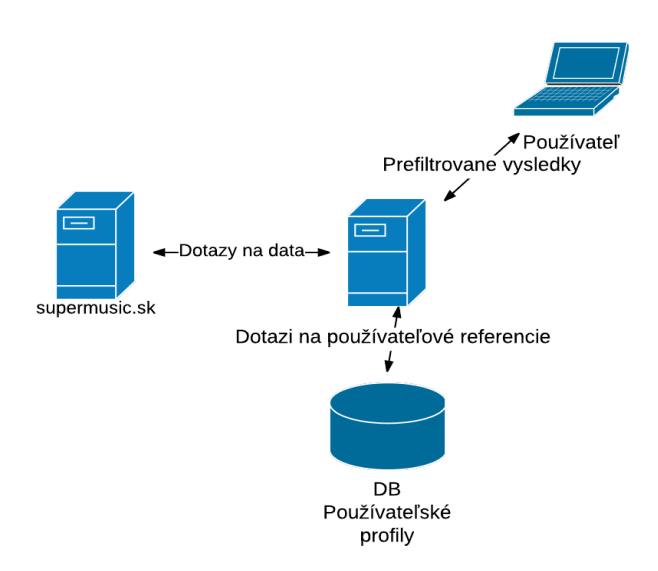
\includegraphics[scale=0.55]{servers}
\caption{Náčrt funkčnosti aplikácie.}\label{Náčrt funkčnosti aplikácie}
\end{center}\end{figure}

\subsection{Zostavenie spevníka}

Aplikácia bude podporovať funkcionalitu automatického generovania spevníka,
kedy si používateľ zvoli používateľov s ktorými si chce ísť zahrať
a aplikácia automatický vygeneruje spevník
zložený s nejpreferovanejších hudobných diel daných používateľov.

\subsection{Krawler ?}

Tento komponenet prehľadáva databázu ktorá je cieľom môjho odporúčača,
využíva k tomu abecedne zobrazenie záznamov databázy.
Databáza sa nedá zobraziť od do,
takže granularitu zobrazenie stránok som musel určiť pokusom,
najskôr som si zobrazoval všetky troj písmenkove názvy,
čo bolo 30*26*26 zobrazení (20280), čo ale trvalo príliš dlho,
tak som v tretej sade prehľadával iba každé štvrté písmenko,
čo zredukovalo počet stranok na 3380.

\subsection{Indexing}

Jestvuje veľa spôsobov ako sa dá označovať a vyhľadať obsah, ja som sa počas prieskumu zameral na try:

\paragraph{Priama tagovacia tabuľka}

Vytvoril som tabuľku tagov, kde bol každý tag fyzický priamo vložený spolu z id dokumentu ku ktoremu sa viaže,
tento prístup ale nebol dostatočne rýchli na vygenerovanie, ani na vyhľadávanie. Pri vyhľadávaní nad 118989 značkamy 
označujúcimi 47002 dokumentov zabral 44.6984 sekúnd. Nepomohlo ani zindexovanie podľa mena.

\paragraph{Model vektorovho priestoru (angl. vector space model}

Pri použití tohto modelu zabral dotaz 0.006 sec.

Tento model sa v MySQL nazýva model prírodzeného jazyka (angl. Natural Language Model),
ktorý porovnáva vlastnosti dokumentov na základe abstrakcie priestoru,
v ktorom sú jednou dimenziou vlastnosti jedného dokuemntu a druhou vlastností druhého
dokumentu, prípade vyhľadávacieho reťazca alebo používateľský profil.
Následne sa vracajú dokumenty ktoré majú najpodobnejší smer vektora k požadovanej fráze.

V MySQL je tento prístup implementovaný pomocov nasledujúcej rovnice \cite{14}:

\[
    w_d = \frac{\log(dtf_d) + 1}{\sum_{i=1}^{t} \log (dtf_i) + 1} .
        \frac{U}{1+0.0115 * U} .
        \log \frac {N}{nf}
\]

\begin{itemize}
\item{\(dtf_d\) je sila (množstvo koľko krát sa nachádza pojem v text v prípade analízy textu)
    vlastnosti vyhodnocovaného dokumentu}
\item{\(dtf_i\) sila i-tej vlastnosti}
\item{\(U\) počet unikátnych vlastnosti dokumentu}
\item{\(N\) počet všetkých dokumentov}
\item{\(nf\) je počet dokumentov ktoré obsahuje danú vlastnosť}
\end{itemize}

Rovnica sa dá rozdeliť na tri časti. 


\paragraph{Základná časť}
Je to primárna rovnica určujúca váhu pojmu.

\paragraph{Normalizačný faktor} 
Spôsobý, že ak je dokument kratší ako preiemerná dĺžka dokuemntu,
jeho relevancia stúpa. \cite{pivoted_doc_len}

\paragraph{Inverzná frequencia}
Zabezpečuje že menej časté pojmy majú vyššiu váhu.

\subsection{Filtrovanie bezvýznamných značiek (angl. stopwords)}

Niektoré slová sú pri vyhľadávaní a indexovaní zbytočné. Síce 
sa dá použiť tf*idf ktorý redukuje váhu slov na základe ich 
unikátnosti, ale tieto slová aj tak musí systém spracovať, ja som 
sa rozhodol použiť kombináciu českých, anglických a slovenských slóv z
projektu TODO: Ako ? google code stop-words

\subsection{Váhovanie Dokumentu}

\[w(d_j) = \sum_{i=1}^{N} w(t_i) \]

\begin{itemize}
\item{\(N\)} Počet značiek v dokumente,
\item{\(t_i\)} I-ty pojem v dokumente,
\item{\(d_j\)} J-ty dokument.
\end{itemize}

%\section{Návrh, špecifikácia požiadaviek a pod.}
%Aenean consequat, sapien a posuere tincidunt, massa purus egestas nisl, sed sollicitudin neque mi vel augue. Sed condimentum nibh ut metus condimentum ornare. Maecenas ultrices tempor condimentum. Etiam nec lorem leo, id consequat tellus. Etiam id mattis massa. Phasellus commodo, lacus in viverra lacinia, quam leo ultricies tellus, condimentum vehicula dui nisl a magna. In mi felis, malesuada eget tincidunt eget, rutrum ac lacus. In a nisl tellus. Mauris hendrerit egestas odio ac consequat. Curabitur aliquam convallis nibh sed blandit. Ut et viverra felis. Sed varius quam non mauris facilisis tincidunt. Quisque et libero eros, sed hendrerit sapien. Aliquam nec faucibus neque. Integer dictum arcu sed risus scelerisque fermentum. Pellentesque vitae ipsum lorem, sed lacinia ligula~\cite{4}.
%
%\begin{figure}\begin{center}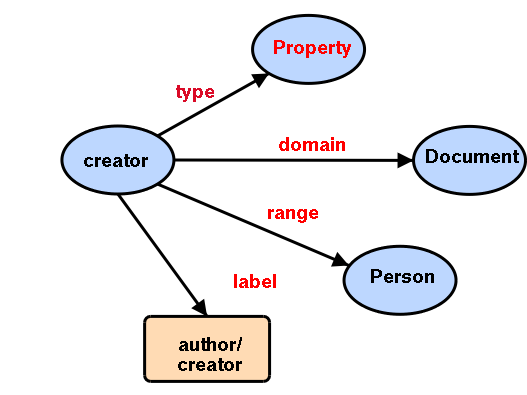
\includegraphics[scale=0.55]{figure2}
%\caption{Popis schémy.}\label{figure2}
%\end{center}\end{figure}
%
%Etiam nec lorem leo, id consequat tellus. Etiam id mattis massa. Phasellus commodo, lacus in viverra lacinia, quam leo ultricies tellus, condimentum vehicula dui nisl a magna. In mi felis, malesuada eget tincidunt eget, rutrum ac lacus. In a nisl tellus. Mauris hendrerit egestas odio ac consequat. Etiam nec lorem leo, id consequat tellus. Etiam id mattis massa. Phasellus commodo, lacus in viverra lacinia, quam leo ultricies tellus, condimentum vehicula dui nisl a magna. In mi felis, malesuada eget tincidunt eget, rutrum ac lacus. In a nisl tellus. Mauris hendrerit egestas odio ac consequat. Etiam nec lorem leo, id consequat tellus. Etiam id mattis massa. Phasellus commodo, lacus in viverra lacinia, quam leo ultricies tellus, condimentum vehicula dui nisl a magna. In mi felis, malesuada eget tincidunt eget, rutrum ac lacus. In a nisl tellus. Mauris hendrerit egestas odio ac consequat.
%
%\lstinputlisting[float=h,language=javascript,caption={Príklad listingu zo súboru.},label={listing},frame=single,frameround=ffff,captionpos=b,basicstyle=\scriptsize]{figures/listing}
%
%Etiam nec lorem leo, id consequat tellus. Etiam id mattis massa. Phasellus commodo, lacus in viverra lacinia, quam leo ultricies tellus, condimentum vehicula dui nisl a magna. In mi felis, malesuada eget tincidunt eget, rutrum ac lacus. In a nisl tellus. Mauris hendrerit egestas odio ac consequat. Etiam nec lorem leo, id consequat tellus. Etiam id mattis massa. Phasellus commodo, lacus in viverra lacinia, quam leo ultricies tellus, condimentum vehicula dui nisl a magna. In mi felis, malesuada eget tincidunt eget, rutrum ac lacus. In a nisl tellus. Mauris hendrerit egestas odio ac consequat. Etiam nec lorem leo, id consequat tellus. Etiam id mattis massa. Phasellus commodo, lacus in viverra lacinia, quam leo ultricies tellus, condimentum vehicula dui nisl a magna. In mi felis, malesuada eget tincidunt eget, rutrum ac lacus. In a nisl tellus. Mauris hendrerit egestas odio ac consequat.
